\section{Results}\label{sec:results}


In this section, we detail the findings of our study.  We remind the reader that our main goal with this study is to
better understand the strengths and limitations of the \mas for malware detection using the state-of-the-art
test case generation tool (DroidBot). We explore
the results of our research using two datasets: the \sds (102 pairs of apps) and the
\cds (\apps pairs of apps).


\subsection{Exploratory Data Analysis of Accuracy}


{\bf \sds.} Considering the \sds (102 apps), the \mas for malware detection 
classifies a total of 69 repackaged versions as malware (67.64\%).
This result is close to what Bao et al. report~\cite{DBLP:conf/wcre/BaoLL18}.
That is, in their
original paper,  the \mas using DroidBot classifies 66.66\% of the
repackaged version of the apps as malware~\cite{DBLP:conf/wcre/BaoLL18}.
This result confirms that we were able to reproduce
the findings of the original study using our
infrastructure. 

\tb{1}{We were able to reproduce the results of
  existing research using our infrastructure,
  achieving a malware classification in the
  \sds close to what has been reported in
  previous studies.}

In the previous studies~\cite{DBLP:conf/wcre/BaoLL18,DBLP:journals/jss/CostaMMSSBNR22},
the authors assume that all repackaged versions contain a
malicious behavior. For this reason, the authors do not
explore accuracy metrics (such as Precision, Recall, and
F-measure ($F_1$))---all repackaged apps labeled as
malware are considered true positives in the previous studies.
As we mentioned, in this paper we take advantage
of \vt to label our dataset and build a ground truth: we only
classify a repackaged version of an app as malware if the results
of our \vt query report that at least two
\ses identify malicious behavior in the asset (again, this
decision follows existing recommendations~\cite{vt-label,DBLP:journals/ese/KhanmohammadiEH19}).
%\kn{Now its a bit clearer, but I would expect a separate paragraph when we introduce VT explaing how VT serves as a better ground truth and also justify our choices on the numbers with VT a bit more -- why we have two as the magic number of antivirus scanners... }
The first row of Table~\ref{tab:accuracy} shows that the \mas achieves an accuracy of 0.89 when
considering the \sds. The \mas fails
to correctly classify seven assets as malware on the \sds (FN column, first row of Table~\ref{tab:accuracy}),
and wrongly labeled the repackaged version of seven apps as malware (FP column).


%\kn{Please re mention in this table the total number of apps in small and complete. Maybe inside the braces as part of the second column entries. }
\begin{table*}[htb]
  \caption{Accuracy of the \mas in both datasets.}
\centering{
  \begin{tabular}{lrrrrrr} \toprule
    Dataset & TP   & FP  & FN  & Precision & Recall & $F_1$ \\ \midrule
    \sds (102)    & 62   & 7   & 7   & 0.89      & 0.89   & 0.89  \\
    %\mas + Traces  & \sds (102)   & 67   & 18  & 2   & 0.78      & 0.97   & 0.87  \\
    \cds (1,707)    & 149  & 249 & 341 & 0.37       & 0.30   & 0.33  \\
    %\mas + Traces  & \cds (1203)   & 214  & 326 & 245 & 0.39      & 0.46   & 0.42  \\ 
    \bottomrule
  \end{tabular}
  }
  \label{tab:accuracy}
\end{table*}

%We also investigate if one could improve the performance of the \mas using an enriched comparison approach. That is, instead of only comparing the sets of calls to sensitive APIs, here we also compare the traces from entry points to such a calls. If there is at least one trace that appears only during the execution of the test cases in the repackaged version of the app, we label that version as a malware.


%Introducing trace analysis reduces the number of false negatives to two, with the side effect of increasing the number of false positives from 7 to 18 (see the second row of Table~\ref{tab:accuracy}). In general, the accuracy ($F_1$) of the \mas using trace analysis drops from 0.89 to 0.87.


%\tb{2}{Although the use of Trace Analysis reduces the number of false negatives (in comparison with the vanilla \mas), it slightly decreases the overall accuracy ($F_1$) of the \mas to detect malware, from 0.89\% to 0.87\% in the \sds.} 



{\bf \cds.} Surprisingly, considering our complete dataset (\apps apps), the \mas
labels a total of 398 repackaged apps as malware (23.31\% of the total number of repackaged
apps)---for which the repackaged version calls at least one additional sensitive API.
Our analysis also reveals a {\bf negative result} related to the accuracy of the approach: here,
the accuracy is much lower in comparison to what we reported for the
\sds (see the second row of Table~\ref{tab:accuracy}): $F_1$ dropping from \fscoreSmall to \fscore.
This result indicates that, when considering a large dataset, the accuracy of the \mas using
DroidBot drops significantly. 

%The use of the trace analysis reduces the number of false negatives in the \cds (from 286 to 245), though increasing the number of false positives from 173 to 326. Altogether, the $F_1$ measure does not change when comparing performance of the vanilla \mas and its trace-based variant in the \cds. 


\tb{2}{
  The \mas for malware detection
  leads to a substantially lower performance on the
  \cds (\apps pairs of apps),
  dropping the accuracy by a factor of 56\%  in comparison to
  what we observed in the \sds.}


Therefore, the resulting sandbox we generate using
DroidBot suffers from a significantly low accuracy rate when considering a
large dataset.
%Besides that, enriching the \mas with trace analysis does not  improve the overall accuracy in the \cds (even though we reduce the number of false negatives with trace analysis, the increasing in the number of false positives negatively impacts the performance of the approach). 
This is shown in the second row of Table~\ref{tab:accuracy}.
The negative performance of the \mas in the \cds encouraged us to endorse efforts aimed at identifying potential reasons for
this phenomenon and motivate the research questions RQ2 and RQ3. 

%\todo[inline]{The previous paragraph now seems a bit unnecessary.}

% \fh{I removed a paragraph here, since it was unncessary}

\subsection{Assessment Based on \sscore}

Figure~\ref{fig:ss} shows the \sscore distribution
over the two datasets we use in our research
(the small and the complete datasets).
Recall that the \sscore measures how similar the
original and repackaged versions of an app are.
The average \sscore of the
\sds is 0.89 (median of 0.99 and sd of 0.25). Contrasting,
the average \sscore of the complete dataset is
0.93 (median of 0.98 and sd of 0.14).

\begin{figure}
  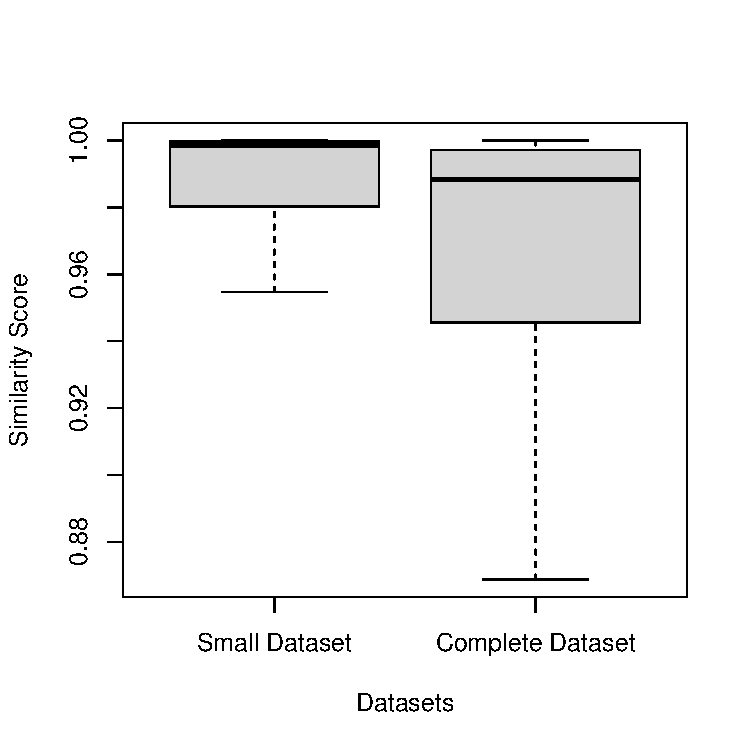
\includegraphics[width=\columnwidth]{images/boxplotSimilarity.pdf}
  \caption{\sscore of the malware samples in the small and complete datasets. The boxplots in the figure do not show
  outliers.}
  \label{fig:ss}
\end{figure}

% \fh{at table 1 I inserted at second columns the sample amount}

Here we hypothesize that \sscore might have an
association with the accuracy of the \mas and could perhaps explain
the differences in the accuracy results we report for both
datasets. We first use Logistic Regression to assess the strength
of the association between label correctness and
the \sscore. To this analysis, we removed the
occurrences of true negatives (i.e., the repackaged version is benign according to
\vt and the \mas correctly label the repackaged version as benign).
As such, we test the following null hypothesis:

\begin{quote}
  {\bf $H_0$} \sscore does not influence the accuracy of the
  \mas for malware detection. 
\end{quote}

The results of the logistic regression suggest that we should
not reject our null hypothesis ($p$-value $<$ 0.89). This finding suggests
that the \mas is not more likely to assign a correct label to
a repackaged app in the cases where its \sscore with the original
app is high (or small). \raw{This is an expected result, since
we found a higher accuracy on the \sds, even though  the
\sscore of the original and repackage apps in both datasets
do not differ significantly.} 

%\kn{I am a bit confused here. Higher similariy score implies the app pairs are close to each other, making the detection easier? Or maybe I misundertood it here.}

\tb{3}{There is no association between
  the \sscore and the \mas performance, which means that
  the similarity between the original and repackaged versions of
  an app is not sufficient to explain the performance
  of the \mas for malware detection.}


\rb{Based on the current results so far, I believe that we should
  remove this study based on k-means}

To clarify the lack of association between
\sscore and correctness, we use the \emph{K-Means} algorithm to split the
\cds into ten clusters---according to the \sscore. We then
estimate the percentage of correct classifications for each cluster, as
we show in Table~\ref{tab:ss-clusters}. Note that the \mas
achieves the highest percentage of correct classification (40.54\%) for the sixth
cluster (cId = 6), which
presents an average \sscore of 0.91\%. Nonetheless, the
cluster cId = 10, with larger number of samples (316) and \sscore (99\%), presents
a percentage of correct classifications around 22\%. 


\begin{table}[ht]
  \caption{Characteristics of the clusters. Note there is no specific
    pattern associating the percentage of
    correct answers with the \sscore.
   For this analysis, we removed the true negatives in our dataset.}
  \centering
  \begin{small}
    \begin{tabular}{rrrrr}   \toprule
 cId & \sscore & Samples & Correct Answers & Percentage \\ \midrule
   1 & 0.02 &  10 &   1 & 10.00 \\ 
   2 & 0.49 &  13 &   2 & 15.38 \\ 
   3 & 0.71 &  14 &   5 & 35.71 \\ 
   4 & 0.80 &  45 &  11 & 24.44 \\ 
   5 & 0.88 &  68 &  10 & 14.71 \\ 
   6 & 0.91 &  37 &  15 & 40.54 \\ 
   7 & 0.94 &  48 &   8 & 16.67 \\ 
   8 & 0.97 &  44 &   8 & 18.18 \\ 
   9 & 0.98 & 144 &  19 & 13.19 \\ 
  10 & 0.99 & 316 &  70 & 22.15 \\ \bottomrule
 \end{tabular}
 \end{small}
 \label{tab:ss-clusters}
 \end{table}


\subsection{Assessment Based on Malware Family}
%\fh{inserted a little introduction about malware family}


%\kn{I feel we need some definition of what we mean by a family of malware. Words like gappusin etc donot have big meaning for people outside this domain}
As we discussed in the previous
section, the similarity assessment does not explain the low performance of the
\mas on the \cds. Since the \cds covers a wide range of malware families, we investigate the
hypothesis that the malware families in the \cds could
explain the poor performance of the \mas on the \cds.
Indeed, in the \cds, we identified a total of
44 families of malwares, though the most frequent
ones are \gps (295 samples), \fm{revmob} (31 samples), \fm{dowgin} (25 samples), and \emph{airpush} (21 samples). Together, they
account for 75.91\% of the repackaged apps in our
complete dataset labeled as malware according to \vt.

This family distribution in the \cds is
different from the family
distribution in the \sds---where the
families \fm{kuguo} (34 samples), \fm{dowgin} (12 samples),
and \fm{youmi} (5 samples) account for
73.91\% of the families considering the 69
repackaged apps \vt labels as malware in the \sds.
Most important, in the \sds, there is just one
sample from the \gps family. This observation
leads us to the question: \emph{how does the \mas
perform when considering only the gappusin samples?}



The confusion matrix of Table~\ref{tab:gappusin} summarizes the accuracy assessment of the \mas considering
only the \gps samples in the \cds. Note that \vt classify as malware all repackaged versions in the \gps
family and that for 269 samples (91.18\%), the \mas was not able to correctly identify
a repackaged version of an app as a malware (recall of 0.08). 
%Merging the outcomes of both approaches (that is, the vanilla \mas and
%the \mas with traces), leads to a recall of
%$\frac{27}{198} = 0.13$. 
Further, if we remove the \gps
samples from the \cds, the recall
of the \mas increases to 0.63 (similar
to the performance of the original studies). 

\begin{table}[ht]
  \caption{Confusion matrix of the \mas when considering only the
  samples from the \gps family in the \cds.}
\centering
\begin{tabular}{r|cc} \hline
\multirow{2}{*}{Actual Condition}   & \multicolumn{2}{c}{Predicted Condition} \\ 
                                    & Benign    & Malware   \\ \hline 
  Benign  (0)                       & TN (0)    & FP (0)    \\
  Malware (295)                     & FN (269)  & TP (26)   \\ \hline
\end{tabular}
\label{tab:gappusin}
\end{table}


\tb{5}{The \mas fails to correctly
  identify 91.18\% of the samples from the \gps family
  as a malware. This is the main reason for the low
  recall of the \mas in the \cds.}

We further analyse the sample of \gps malware in our dataset, given its
relevance to the negative result we present in our paper. First,
Figure~\ref{fig:hist-gappusin} shows a histogram of the \sscore for the samples
in the \gps family. Note that mostly of the repackaged versions from the
\gps family are quite similar to the original versions (average \sscore
of 0.97, median \sscore of 0.99, and sd of 0.06). We also reengineer
a sample of 30 \gps malware (more than 10\% of the samples in this
family), using the \texttt{SimiDroid}\footnote{https://github.com/lilicoding/SimiDroid},
\texttt{apktool}~\footnote{https://ibotpeaches.github.io/Apktool/},
and \texttt{smali2java}~\footnote{https://github.com/AlexeySoshin/smali2java} tools.
Considering this sample of 30 \gps malware, the median \sscore is \raw{0.99}. In addition,
the repackaged version of the apps changes \raw{4.96} methods (on average). Table~\ref{tab:simidroid-outputs} summarizes
the outputs of \texttt{SimiDroid} for this sample of \gps apps.

The similarity assessment of this sample of 30 \gps malware reveals a few modification patterns when comparing the original and the
repackaged versions of the apps. First, no instance in this \gps sample dataset
modifies the Android Manifest file to require additional permissions, for instance.
In most of the cases, the repackaged version just changes the Manifest file to modify either
the package name or the main activity name. Moreover, 29 out of the 30 samples in this dataset  {\bf modifies} the 
method \texttt{void onReceive(Context,Intent)>} of the class \texttt{com.games.AdReciver}. Although the results of the
decompilation process are difficult to understand in full (due to code obfuscation),
the goal of this modification is to change the behaviour of the benign version, so that it can
download a different version of the \texttt{data.apk} 
asset. Figure~\ref{code:onReceive} shows
the code pattern of the \texttt{onReceive} method presents in the samples. This modification
typically use a new method (\texttt{public void a(Context)}
the repackaged versions often introduce into the same class (\texttt{AdReciver}).
Since there is no extra call to sensitive APIs, the \mas fails to label
the \gps samples correctly. 

.
%\begin{wrapfigure}{l}{0.4\textwidth}
\begin{figure}
\begin{center}
    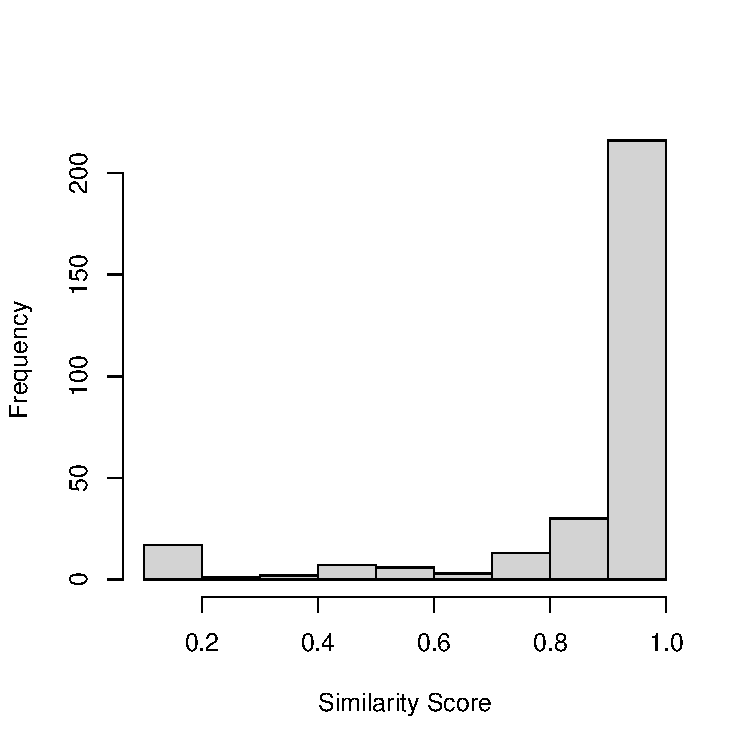
\includegraphics[width=0.38\textwidth]{images/similarityGappusin.pdf}
  \end{center}
  \caption{Histogram of the \sscore for the samples in the \gps family.}
  \label{fig:hist-gappusin}
\end{figure}  
%\end{wrapfigure}

\begin{figure*}
\begin{lstlisting}[language=Java]
public void onReceive(Context context, Intent intent) {
  SharedPreferences sp = context.getSharedPreferences(String.valueOf("com.") + "game." + "param", 0);
  int i = sp.getInt("sn", 0) + 1;
  System.out.println("sn: " + i);
  if (i < 2) {
    mo4a(context);
    SharedPreferences.Editor edit = sp.edit();
    edit.putInt("sn", i);
    edit.commit();
  } else if (!new C0004b(context).f7h.equals("")) {
    String str1 = context.getApplicationInfo().dataDir;
    String str2 = String.valueOf(str1) + "/fi" + "les/d" + "ata.a" + "pk";
    String str3 = String.valueOf(str1) + "/files";
    String str4 = String.valueOf("com.") + "ccx." + "xm." + "SDKS" + "tart";
    String str5 = String.valueOf("InitS") + "tart";
    String str6 = "ff048a5de4cc5eabec4a209293513b6e";    
    C0003a.m3a(context, str2, str3, str4, str5, str6);
    SharedPreferences.Editor edit2 = sp.edit();
    edit2.putInt("sn", 0);
    edit2.commit();
  }
}
\end{lstlisting}
\caption{Method introduced in 29 out of 30 \gps malware we randomly selected from the \cds.}
\label{code:onReceive}
\end{figure*}

Our assessment also reveals recurrent modification patterns that {\bf delete} methods in the
repackaged version of the apps. For instance, 20 repackaged apps in our
\gps sample of 30 malware remove the method \texttt{void b(Context)} from the
class \texttt{com.game.a}. This class extensively use 
the Android reflection API. Although it is not clear the real purpose of removing these methods,
that decision simplifies the procedure of downloading a \texttt{data.apk} asset that is different
from the asset available in the original version of the apps. Removing those methods might
also be an strategy for antivirus evasion. For instance, although
some usages of the class \texttt{DexClassLoader} might be legitimate, it allows specific
types of atack based on dynamic code injection~\cite{falsina:acsac}. As such, 
antivirus might flag specific patterns using the Android reflection API suspect. 
Unfortunately, the \mas also fails to identify
a malicious behavior with this type of change (i.e., changes that remove methods).
Listing~\ref{code:deletedMethod} shows an example of code pattern frequently removed
from the repackaged versions from the \gps family. 

\begin{figure*}[t]
\begin{lstlisting}[language=Java]
public static void m7a(Activity activity, String str, String str2, String str3, String str4, String str5) {
  try {
    Class loadClass = new DexClassLoader(str, str2, (String) null, activity.getClassLoader()).loadClass(str3);
    Object newInstance = loadClass.getConstructor(new Class[0]).newInstance(new Object[0]);
    Method method = loadClass.getMethod(str4, new Class[]{Activity.class, String.class});
    method.setAccessible(true);
    method.invoke(newInstance, new Object[]{activity, str5});
  } catch (Exception e) {
    e.printStackTrace();
  }
}  
\end{lstlisting}
\caption{Example of method that is typically removed from the repackaged apps of the \gps family.}
\label{code:deletedMethod}
\end{figure*}

 
\begin{table}[ht]
  \centering
  \caption{Summary of the outputs of the \texttt{SimiDroid} tool for the sample of 30
    \gps malware. (IM) Identical Methods, (SM) Similar Methods, (NM) New Methods, and
    (DM) Deleted Methods.}
  \begin{tabular}{lrrrrr}
    \toprule
 Hash  & \sscore &   IM  &   SM  &  NM   &  DM  \\ \midrule
 33896E & 0.9994 &  3205 &     2 &     0 &     0 \\ 
 0C962D & 0.9994 &  3413 &     1 &     1 &    10 \\ 
 BCDF91 & 0.9992 &  2645 &     2 &     0 &     0 \\ 
 01ECE4 & 0.9991 &  5697 &     4 &     1 &    10 \\ 
 A306DA & 0.9989 &  1886 &     1 &     1 &     6 \\
 4010CA & 0.9987 &  3721 &     1 &     4 &     6 \\
 5B5F2D & 0.9983 &  1164 &     2 &     3 &     0 \\
 010C07 & 0.9982 &  2248 &     4 &     3 &     0 \\
 F9FC04 & 0.9982 &  1121 &     1 &     1 &     6 \\
 E29F53 & 0.9976 &   842 &     1 &     1 &     6 \\
 FE76EB & 0.9976 &   839 &     1 &     1 &     6 \\
 842BD5 & 0.9973 &  2249 &     3 &     3 &     3 \\
 295B66 & 0.9972 &  1081 &     2 &     1 &    10 \\
 92209D & 0.9971 &   698 &     2 &     3 &     0 \\
 0977B0 & 0.9969 &  1613 &     4 &     1 &    10 \\
 347FCF & 0.9967 &   613 &     1 &     1 &     6 \\
 00405B & 0.9965 &   864 &     2 &     1 &    10 \\
 67310E & 0.9957 &  1164 &     2 &     3 &     3 \\
 CCD29E & 0.9954 &   436 &     2 &     0 &     0 \\
 610113 & 0.9941 &   836 &     4 &     1 &    10 \\
 A871E0 & 0.9941 &   836 &     4 &     1 &    10 \\
 ECEA10 & 0.9913 &   229 &     1 &     1 &     6 \\
 E53FAA & 0.9889 &   267 &     2 &     1 &    10 \\
 723C23 & 0.9870 &   228 &     2 &     1 &    10 \\
 D95B6E & 0.9870 &   833 &    10 &     1 &    10 \\
 17722D & 0.9743 &   265 &     6 &     1 &    10 \\
 537492 & 0.9504 &   134 &     6 &     1 &    10 \\
 078E0A & 0.9504 &   134 &     6 &     1 &    10 \\
 D83F1C & 0.9494 &   150 &     2 &     6 &     6 \\
 E5D716 & 0.8840 &  2035 &    68 &   199 &   199 \\ 
   %% \texttt{0C962D289E}&0.933&99&7&0&0 \\
%% \texttt{E5D71699E7}&0.971&275&8&0&0 \\
%% \texttt{ECEA10902B}&0.897&44&5&0&0 \\
%% \texttt{5374927E98}&0.974&349&9&0&0 \\
%% \texttt{E29F53DA37}&0.986&375&5&0&0 \\
%% \texttt{BCDF919487}&0.982&334&6&0&0 \\
%% \texttt{01ECE4AE23}&0.931&108&6&2&2 \\
%% \texttt{610113BB0C}&0.964&192&7&0&0 \\
%% \texttt{295B663AD1}&0.946&196&11&0&0 \\
%% \texttt{17722D9807}&0.867&46&7&0&0 \\
%% \texttt{67310E41EC}&0.956&154&5&2&2 \\
%% \texttt{5B5F2D5DAA}&0.956&154&5&2&2 \\
%% \texttt{F9FC043249}&0.925&148&12&0&0 \\
%% \texttt{010C070CAD}&0.968&245&6&2&2 \\
%% \texttt{842BD5F8A9}&0.972&246&5&2&2 \\
%% \texttt{00405B66DD}&0.835&66&13&0&0 \\
%% \texttt{D83F1CEA61}&0.901&73&6&2&2 \\
%% \texttt{723C231BA7}&0.857&42&7&0&0 \\
%% \texttt{33896EBEC0}&0.978&229&5&0&0 \\
%% \texttt{347FCF5AC1}&0.956&110&5&0&0 \\
%% \texttt{4010CA0E70}&0.917&78&5&2&2 \\
%% \texttt{D95B6E6417}&0.981&373&7&0&0 \\
%% \texttt{A871E01516}&0.964&192&7&0&0 \\
%% \texttt{CCD29EC8ED}&0.953&102&5&0&0 \\
%% \texttt{FE76EBE7B4}&0.974&194&5&0&0 \\
%% \texttt{A306DA6482}&0.853&35&6&0&0 \\
%% \texttt{E53FAABBA0}&0.941&162&10&0&0 \\
%% \texttt{92209D0E67}&0.975&284&5&2&2 \\
%% \texttt{078E0AE6E3}&0.977&350&8&0&0 \\
%% \texttt{0977B0E411}&0.946&196&9&2&2 \\
   \bottomrule
 \end{tabular}
 \label{tab:simidroid-outputs}
\end{table}

In summary, our reverse engineering effort brings evidence that malware
samples from the \gps family neither modify the Android Manifest
files nor call additional sensitive APIs---which reduce the ability
of the \mas to correctly classify a sample as a malware. We argue in favor
of new research efforts to integrate the \mas 
with other techniques that could increase their performance
on malware identification. Since the samples from the \gps
family use specific patterns to introduce malicious behavior,
it might be promising to explore static analysis approaches that
search for these specific patterns. 

%% \kn{I really like this part of the gps family analysis. }



%% %% \begin{figure}
%% %%   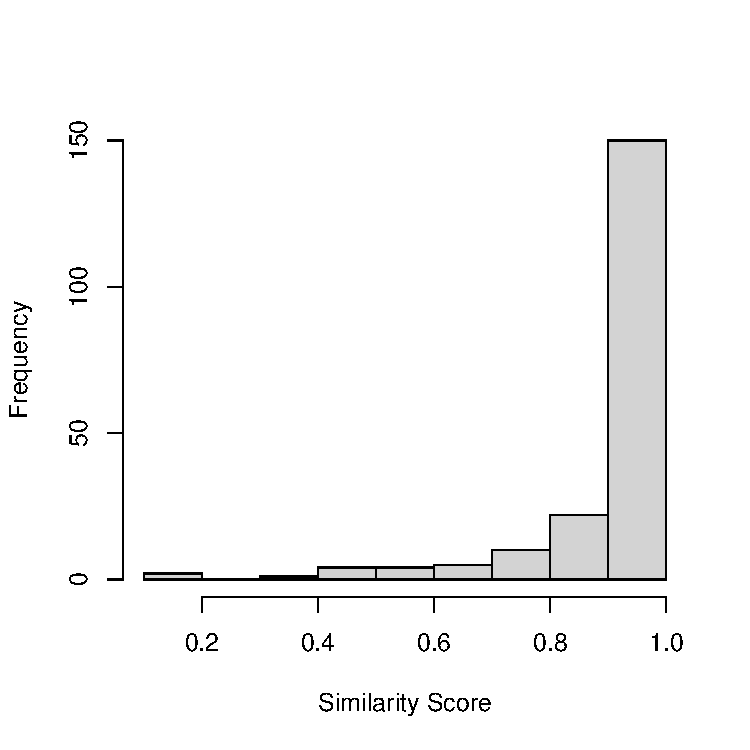
\includegraphics[scale=0.5]{images/gappusin-1.pdf}
%% %% \end{figure}

%% \todo[inline]{{\bf RB}. Removing the \gps family improves
%%   the recall, though did not improve precision. What is the reason
%%   for the low precision of \mas in the \cds? We should investigate
%% this issue.}


%% Considering
%% manifest analysis, as we explained in Section~\ref{sec:manifestAnalysis},
%% looking at the occurrence of duplicated permissions and duplicated 
%% components allows us to correctly classify \num{120} out of the \num{607} missed cases
%% from the mining sandbox approach (\num{19.76}\%).                                   
%% Table~\ref{tab:mfa-complete} summarizes the results of this investigation. When considering the 
%% complete dataset (\num{800} apps), combining the vanilla
%% mining sandbox approach (VMS) with trace analysis (TA) and
%% manifest analysis (MA) leads to the correct classification
%% of \num{446} malware (\num{55.75}\%), which suggests that
%% the mining sandbox approach requires further improvements when
%% we take into account a more representative dataset
%% of malware. 


%% \begin{table}[ht]
%%   \centering
%%   \begin{small}
%%   \begin{tabular}{lcc}\toprule
%%   Technique      & Hits & Recall \\ \midrule 
%%   VMS            & 193  & \num{24.12}\% \\ 
%%   VMS + TA       & 369  & \num{46.12}\%  \\
%%   VMS + MA       & 313  & \num{39.12}\% \\
%%   VMS + TA + MA  & 446  & \num{55.75}\% \\  \bottomrule
%%   \end{tabular}
%%   \end{small}
%%     \caption{Summary of the results in the Complete Dataset.}

%%  \label{tab:mfa-complete}
%% \end{table}

%% \begin{obs}{5}{}
%%   The results so far bring evidence that
%%   further research is necessary to understand
%%   the limitations of the mining sandbox approach
%%   targeting more comprehensive datasets.
%% \end{obs}

%% Our exploration of all sensitive APIs called by all app pairs brought to the light the most frequently abused sensitive APIs that
%% appear in the repackaged, malicious version of the apps. We observed that when executed all 800 app pairs, DroidBot called $75$ sensitive APIs at least one time (from our list of 162 sensitive APIs). Among them, $16$ APIs account for more than half of all calls ($51.06$\%).
%% %\rb{I could not understand the previous sentence}.
%% The sensitive API that is abused the most by repackaged apps is \textbf{android.telephony.TelephonyManager: java.lang.String getDeviceId()}, which gets the device
%% IMEI\footnote{From Wikipedia: International Mobile Equipment Identity (IMEI) is a number, usually unique, to identify 3GPP and iDEN mobile phones.}.
%% Table~\ref{tab:APIused} presents the list of the most frequent sensitive APIs that only the malicious
%% version of the apps in our dataset call.

%% \begin{obs}{6}{}
%%   The results so far bring evidence that only a handful of resources accesses like the \textbf{device id} are most attractive to malware designers, providing a potentially high-impact point of focus for future researchers and practitioners.
%% \end{obs}

%% %\begin{landscape}
%% \begin{table*}[t]
%%  \scriptsize
%%   \caption{Sensitive APIs more used by repackage apps}
%%   \centering
%%   %\begin{small}
%%  \begin{tabular}{lc}

%%    \toprule
%%    Sensitive API & Occurrences \\
%%    \midrule
%%    01 android.telephony.TelephonyManager: java.lang.String getDeviceId() &  78 \\
%%    02 android.net.wifi.WifiManager: android.net.wifi.WifiInfo getConnectionInfo() &  64\\
%%    03 android.net.wifi.WifiInfo: java.lang.String getMacAddress() &  63 \\
%%    04 android.net.NetworkInfo: java.lang.String getTypeName() &  58 \\
%%    05 android.net.NetworkInfo: java.lang.String getExtraInfo() &  56 \\
%%    06 android.telephony.TelephonyManager: java.lang.String getSubscriberId() &  54 \\
%%    07 android.net.NetworkInfo: android.net.NetworkInfo State getState() &  52 \\
%%    08 android.database.sqlite.SQLiteOpenHelper: android.database.sqlite.SQLiteDatabase getWritableDatabase() &  49 \\
%%    09 android.database.sqlite.SQLiteDatabase: android.database.Cursor query(java.lang.String, ...,java.lang.String) &  47 \\
%%    10 android.telephony.TelephonyManager: java.lang.String getNetworkOperator() &  45\\
%%    11 android.telephony.TelephonyManager: android.telephony.CellLocation getCellLocation() &  44\\
%%    12 android.database.sqlite.SQLiteOpenHelper: android.database.sqlite.SQLiteDatabase getReadableDatabase() &  44\\
%%    13 android.telephony.gsm.GsmCellLocation: int getLac() &  42 \\
%%    14 android.telephony.gsm.GsmCellLocation: int getCid() &  42 \\
   
%%    15 android.net.ConnectivityManager: android.net.NetworkInfo getNetworkInfo(int) &  39 \\
%%    16 android.telephony.TelephonyManager: java.lang.String getNetworkOperatorName() &  36 \\
%%    .&  .\\
%%    .&  .\\
%%    .&  .\\
%%    74 android.app.ActivityManager: java.util.List getRecentTasks(int,int) & 1 \\
%%    75 android.net.NetworkInfo: java.lang.String toString() & 1 \\

%%  \bottomrule
%%                             Total & 1592 \\

%%  \end{tabular}
%%  %\end{small}
%%  \label{tab:APIused}
%% \end{table*}
%\end{landscape}

%% \begin{obs}{1}{}
%%    %\kn{Here we need to add some final take aways of the reproduction study}
%%    Our results indicate that in the presence of a representative dataset ($800$ app pairs as opposed to $102$ and a diverse similarity index), the accuracy of state of the art in mining sandbox approaches, using DroidBot drops significantly (from $63.36\%$ to $24.12\%$). Our results also indicate that only few sensitive APIs are responsible for majority of injected malware in repackaged apps. This encourages the emergence of new proposals that can support mine sandbox mitigating \textit{blindspot}s that lead to low accuracy.
%%  \end{obs}


%\kn{In this subsection, are we simply reproducing the results of existing papers. Because as far as I understand, tools like DroidBOT etc. were evaluated by simply comparing the sensitive APIs call. I am guessing here our contribution is to evaluate it on the larger dataset. I have given it a shot, please keep me posted if this is correct.}

%% \subsection{Trace Analysis Results}\label{sec:traceResults}

%% In this section, we describe the results of our investigation on how the trace from the entry point to sensitive API could impact the accuracy of sandbox approaches. Initially, we collect the call graphs of DroidBot execution using \emph{Logcat} and filter in the traces between the app's entry point and calls to any sensitive methods.

%% Then, using the callgraph from executions of both app versions (benign/malicious), we track the differences between their traces. We choose to investigate only app pairs that covered the same set of sensitive APIs detected in both versions during our first experiment (Section~\ref{sec:Sensitive APIs}). 


%% \begin{obs}{2}{}
%%  The state of the art in mining sandbox approaches using DroidBot have a blind-spot when it comes to being aware of the trace taken from the entry point to a sensitive API call. The approaches could have a improvement of $22\%$ if it considered trace as a factor. Similar  improvements are also seen with the original dataset of $101$ app pairs (improvement of $18.81\%$).
%%  \end{obs}

%% \subsection{Manifest File Analysis}\label{sec:manifestResults}

%% In this section, we describe the results of our investigation on the impact of modified manifest files on the accuracy of sandbox approaches. 
%% To this end, we check some particulars from manifest file, that point to a likely suspicious behavior. In section \ref{sec:manifestAnalysis}, we illustrated that an automatic hacking script could inject permission requests at manifest file regardless of whether this request is already present on it, which can result in duplicated permission and actions in the Manifest file. We looked out for such modifications in the malware that went undetected by the test generation tools. Table~\ref{tab:mfa} summarizes our results.


%% The column (SAPI) indicates the number of malware that went undetected during our first study (same as Table~\ref{tab:pa}'s Same API set (SAPI)). The second column (DP) indicates how many Manifest files from malicious app undetected at first study, had duplicated permission. Same way, column (DA) denotes the number of Manifest files with the duplicated actions in their manifest file.

%% A duplicate request for permission or action in a malicious version's manifest file should have been performed by a script. A simple analysis of manifest file could detect $120$ of undetectable malware from the first experiment ($607$), if it considers explorer duplicate permissions or actions at manifest file code as a detection strategy. If we combine the previous trace analysis with manifest file analysis, we improve the accuracy rate to $55.75\%$.

%% It is to be noted that in the presence of the original dataset of $101$ app pairs, the manifest file analysis combined with the trace analysis earlier discussed improves the accuracy rate to $90.09\%$ confirming that such an analysis, even though naive and simple does have an impact on the accuracy rate of mining sandbox approaches.  %\kn{Handrick as before please put the full numbers in the table}


%% \begin{obs}{3}{}
%%  We can conclude that sandbox approach also could have better accuracy if they considered the suspicious modifications in manifest file in their analysis. Although the analysis required of the manifest file is quite naive, we believe the results present an interesting and relevant insight for developers of malware detection tools to improve accuracy.
%% \end{obs}

%% \todo[inline]{rb: I reviewed the paper until this point. I think that next we should
%% provide more explicit answers to the research questions. kn: Given this a shot}

%% \todo[inline]{mm: any finding we want to formulate related to the discussion in the last paragraph? kn: Given it a shot}

